\newcommand{\xbr}{\left(x\right)}
\newcommand{\br}[1]{\left(#1\right)}

\chapter{The model}

The system being under consideration consists of two 1D s-type superconducting wires connected with a tunnel junction. Also  there is a strong spin-orbit coupling assumed to be present and external magnetic field is applied in the direction perpendicular to the wire. The Hamiltonianm of the bulk of each wire, written in the Bogoliubov-de Gennes formalism, is similar to the ones presented in \cite{Oreg_2010} and \cite{Lutchyn_2010}:

\begin{gather}
	\mathcal{H}
	=
	\int dy ~
	\Psi^\dagger
	\br{y}
	H
	\Psi
	\br{y}
	\
	~~~~
	\Psi
%	\left(x\right)
	=
	\begin{pmatrix}
		\psi_\uparrow
		\\
		\psi_\downarrow
		\\
		\psi_\downarrow^\dagger
		\\
		-\psi_\uparrow^\dagger
	\end{pmatrix}
	\\
	\label{bulk_Hamiltonian}
	H
	=
	\br{
		\frac{p^2}{2m}
		-\mu_0
	}\tau_z
	+
	u p \sigma_z \tau_z
	+
	B\sigma_x	
	+
	\Delta\tau_\phi
\end{gather}

Here $ \sigma_i $ and $ \tau_i $ are Pauli matrices in spin and particle-hole subspaces respectfully, $ \tau_\phi = \tau_x \cos\phi - \tau_y \sin_\phi$ with $ \phi $ being a superconducting phase, $ \mu_0 $ is a chemical potential, $ B $ is an external magnetic field, $ \Delta $ is the module of superconducting order parameter and $ u $ is spin-orbit coupling constant with the dimension of velocity. The wire is being aligned along the y-axis, while the direction of the magnetic field coincides with x-axis. Note, that only one component of from spin-orbit is nonzero due to 1D nature of the problem.

The tunnel junction is introduced  by applying an external electrical field. To take it into account it's necessary to include additional term  $ U \br{y}\tau_z $ in (\ref{bulk_Hamiltonian}). However this term can be combined with the chemical potential by introducing $ \mu \br{y} = \mu_0 - U\br{y} $.

\begin{figure}
	\centering
	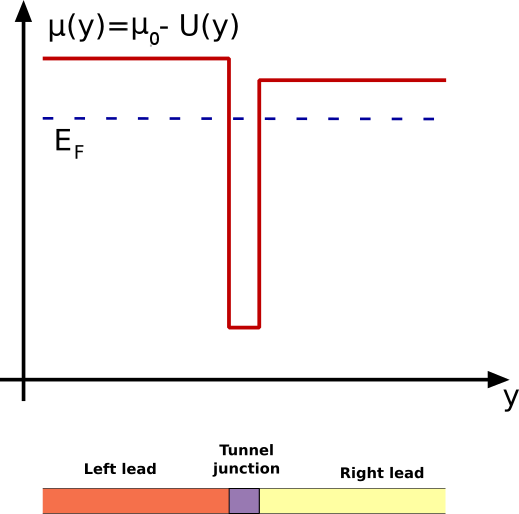
\includegraphics[width=0.7\linewidth]{images/chem_potential}
	\caption{}
	\label{fig:chempotential}
\end{figure}


It can be argued, that superconducting correlations are not possible in thin wires due to the presence of fluctuations. However in real systems this difficulty can be avoided with the help of the proximity effect. The wire itself is assumed to be metallic or semiconductor, and being put close to a strong superconductor. Due to proximity effect it's possible to obtain a presence of order parameter inside initially nonsuperconducting wire.